\documentclass[border=4pt]{standalone}
% Preámbulo común de las figuras. Cada figura es un documento standalone
% que se compila a SVG con scripts/build_figures.sh
\usepackage[utf8]{inputenc}
\usepackage{amsmath}
\usepackage{tikz}
\usepackage[american, siunitx]{circuitikz}
\usetikzlibrary{arrows.meta,calc,decorations.pathmorphing,patterns}
\tikzset{
  >={Stealth[length=2.2mm]},
  eje/.style={->, thin},
  hilo/.style={thick},
}
% Paleta común: tonos medios legibles sobre fondo claro
\definecolor{azul}{RGB}{31,94,168}
\definecolor{rojo}{RGB}{192,57,43}
\definecolor{verde}{RGB}{39,128,73}
\definecolor{naranja}{RGB}{211,120,30}
\definecolor{morado}{RGB}{125,60,152}

\begin{document}
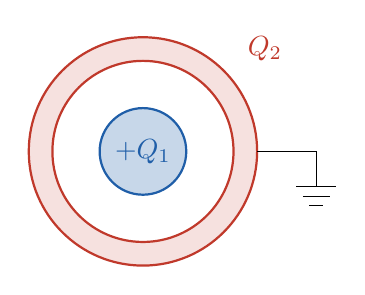
\begin{tikzpicture}[scale=1.0]
  \filldraw[draw=rojo, fill=rojo!15, thick, even odd rule] (0,0) circle (1.45) (0,0) circle (1.15);
  \filldraw[draw=azul, fill=azul!25, thick] (0,0) circle (0.55);
  \node[text=azul] at (0,0) {$+Q_1$};
  \node[text=rojo] at (1.55,1.3) {$Q_2$};
  \draw (1.45,0) -- (2.2,0) -- (2.2,-0.45);
  \draw (1.95,-0.45) -- (2.45,-0.45) (2.03,-0.57) -- (2.37,-0.57) (2.11,-0.69) -- (2.29,-0.69);
\end{tikzpicture}
\end{document}
